\documentclass{standalone}
\usepackage{../../../../preamble_formulas}

\begin{document}
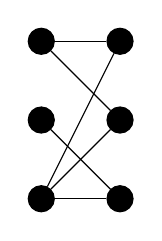
\begin{tikzpicture}
  \foreach \i [count=\X] in {(0,1), (0,0), (0,-1)}{
      \node (\X) at \i  [shape=circle,draw=black,radius=0.5cm,\apl,fill=\apl] {};
    }
  \foreach \i [count=\X starting from 4] in {(1,1), (1,0), (1,-1)}{
      \node (\X) at \i  [shape=circle,draw=black,radius=0.5cm,\ana,fill=\ana] {};
    }


  \path  (1) edge (4);
  \path  (1) edge (5);
  \path  (2) edge (6);
  \path  (3) edge (4);
  \path  (3) edge (5);
  \path  (3) edge (6);
\end{tikzpicture}
\end{document}